\documentclass[conference]{IEEEtran}

\ifCLASSINFOpdf
\else
\fi
\hyphenation{op-tical net-works semi-conduc-tor}

\input{00setup/preambleIEEE.tex}
\usepackage{schemabloc}
\usetikzlibrary{shapes,arrows}
\usepackage{pgfplots}
\usetikzlibrary{plotmarks}
\pgfplotsset{compat=newest}
\pgfplotsset{filter discard warning=false}

\usetikzlibrary{external}
\tikzexternalize[prefix=tikz/]
\pgfdeclarelayer{bg}    % declare background layer
\pgfsetlayers{bg,main}


%\usepackage{silence}
%\WarningsOff[pgfplots]
%\WarningFilter{latex}{Marginpar on page}
%\WarningsOff[latex]


%%% Tikz Magic %%%
\tikzstyle{block} = [draw,rounded corners , rectangle, minimum height=3em, minimum width=6em]
\tikzstyle{Integrator} = [draw, fill=blue!20, rectangle, minimum height=5mm, minimum width=5mm]
\tikzstyle{Twolineblock} = [draw,rounded corners , rectangle, minimum height=3em, minimum width=6em, text width = 6em, align=center]     
\tikzstyle{sum} = [draw, fill=blue!20, circle, node distance=1cm]
\tikzstyle{input} = [coordinate]
\tikzstyle{output} = [coordinate]
\tikzstyle{pinstyle} = [pin edge={to-,thin,black}]
\tikzstyle{box} = [draw,rounded corners, minimum height=15mm, minimum width=20mm, align=center, text centered]
\tikzstyle{BlackBox} = [draw, fill=black, rounded corners, minimum height=15mm, minimum width=20mm, align=center, text=white, text centered]
\tikzstyle{FlowIF} = [diamond, draw, fill=blue!20, text width=8.5em, text badly centered, node distance=3cm, inner sep=0pt,align=center,aspect=3]
\tikzstyle{FlowBlock} = [rectangle, draw, fill=blue!20, text width=8em, text centered, rounded corners, minimum height=3em]
\tikzstyle{FlowCloud} = [draw, ellipse,fill=red!20, node distance=3cm, minimum height=2em]
\tikzstyle{TestBox} = [rectangle,draw, fill=black!20, minimum height=8mm, minimum width=8mm]
\tikzstyle{TestDiamond} = [diamond, draw, fill=black!20, minimum height=10.5mm, minimum width=10.5mm]
\tikzstyle{TestBox} = [rectangle,draw, fill=black!20, minimum height=8mm, minimum width=8mm]
\tikzstyle{TestCircle} = [circle, draw, fill=black!20, minimum height=6mm, minimum width=6mm]
\tikzstyle{TestTable} = [rectangle, draw, fill=black!60, minimum height=0.01mm, minimum width=9mm, text=white]
\tikzstyle{TestBoxSmall} = [rectangle,draw, fill=black!, minimum height=8mm, minimum width=8mm,text=white]
\tikzstyle{LegendBox} = [rectangle,draw, minimum height=7mm, minimum width=20mm]
\tikzstyle{Sysbox} = [draw,rounded corners, minimum height=15mm, minimum width=9em, align=center, text centered,text width = 10.5em]
\tikzstyle{SysBlackBox} = [draw, fill=black, text=white, rounded corners, minimum height=15mm, minimum width=9em, align=center, text centered,text width = 10em]
\tikzstyle{PreAmpBox} = [rectangle,draw, fill=black!20, minimum height=8mm, minimum width=12mm]
\tikzstyle{gain} = [fill=white, draw, rectangle, minimum height=2.5em, minimum width=2.5em]
\tikzstyle{summation} = [draw, minimum size=0.75cm, circle, node distance=1.75cm]












%% Its a pie chart!! %%%
\definecolor{rosso}{RGB}{220,57,18}
\definecolor{giallo}{RGB}{255,153,0}
\definecolor{blu}{RGB}{102,140,217}
\definecolor{verde}{RGB}{16,150,24}
\definecolor{viola}{RGB}{153,0,153}

\makeatletter

\tikzstyle{chart}=[
    legend label/.style={font={\scriptsize},anchor=west,align=left},
    legend box/.style={rectangle, draw, minimum size=5pt},
    axis/.style={black,semithick,->},
    axis label/.style={anchor=east,font={\tiny}},
]

\tikzstyle{bar chart}=[
    chart,
    bar width/.code={
        \pgfmathparse{##1/2}
        \global\let\bar@w\pgfmathresult
    },
    bar/.style={very thick, draw=white},
    bar label/.style={font={\bf\small},anchor=north},
    bar value/.style={font={\footnotesize}},
    bar width=.75,
]

\tikzstyle{pie chart}=[
    chart,
    slice/.style={line cap=round, line join=round, very thick,draw=white},
    pie title/.style={font={\bf}},
    slice type/.style 2 args={
        ##1/.style={fill=##2},
        values of ##1/.style={}
    }
]

\pgfdeclarelayer{background}
\pgfdeclarelayer{foreground}
\pgfsetlayers{background,main,foreground}



\newcommand{\pie}[3][]{
    \begin{scope}[#1]
    \pgfmathsetmacro{\curA}{90}
    \pgfmathsetmacro{\r}{1}
    \def\c{(0,0)}
    \node[pie title] at (90:1.3) {#2};
    \foreach \v/\s in{#3}{
        \pgfmathsetmacro{\deltaA}{\v/100*360}
        \pgfmathsetmacro{\nextA}{\curA + \deltaA}
        \pgfmathsetmacro{\midA}{(\curA+\nextA)/2}

        \path[slice,\s] \c
            -- +(\curA:\r)
            arc (\curA:\nextA:\r)
            -- cycle;
        \pgfmathsetmacro{\d}{max((\deltaA * -(.5/50) + 1) , .5)}

        \begin{pgfonlayer}{foreground}
        \path \c -- node[pos=\d,pie values,values of \s]{$\v\%$} +(\midA:\r);
        \end{pgfonlayer}

        \global\let\curA\nextA
    }
    \end{scope}
}

\newcommand{\legend}[2][]{
    \begin{scope}[#1]
    \path
        \foreach \n/\s in {#2}
            {
                  ++(0,-10pt) node[\s,legend box] {} +(5pt,0) node[legend label] {\n}
            }
    ;
    \end{scope}
}

\begin{document}

\title{Active Noise Control of Speech in Headphones using Linear Prediction}

\author{\IEEEauthorblockN{Mikkel Krogh Simonsen, Kasper Kiis Jensen, Maxime Démurger, Oliver Palmhøj Jokumsen, \\ Christian Claumarch}
\IEEEauthorblockA{Aalborg University - Acoustics and Audio Technology - 1$^{st}$ Semester \\
\{mksi13, kkje13, ojokum12, cclaum16, mdemur16\}@student.aau.dk}
}

\maketitle

\begin{abstract}
Active Noise Control (ANC) is a widely used technique. However most solutions are targeted at attenuating static noise with limited bandwidth. This paper focusses on using prediction to improve attenuation for non stationary signals.
The solution proposed uses an FIR-filter adapted by an Filtered-$x$ Least Mean Square (FXLMS)-algorithm combined with Linear Prediction (LP) to attenuate a speech signal. This solution uses the quasi-periodic properties of speech to estimate the upcoming content of a speech signal. Thereby decreasing the sample delay in the system which increases bandwidth, yielding better attenuation.
\end{abstract}

\IEEEpeerreviewmaketitle

%% Introduction
\section*{Introduction}
\lettrine[lines=2]{A}{ctive} Noise Control (ANC) is becoming a widely used technique in consumer headphones to attenuate external noise. A parameter in ANC is the bandwidth which is determined by the system delay, introduced by sampling and processing the signal in the feedforward system. Consumer ANC headphones has a bandwidth that does not cover the entire frequency area of speech. This paper examines how to extend the bandwidth.

The general solutions in ANC are described thoroughly by Hansen et al. \cite{Hansen2}, \cite{Hansen}. The solution used as a reference in this paper is the digital feedforward system using the Filtered-X Least Mean Squares (FXLMS) method. To increase bandwidth a prediction algorithm is proposed as a potential solution. In order to do prediction, certain signal characteristics must be known, here speech is chosen as the noise source. Prediction of speech is described by Wai C. Chu \cite{Speech}. In this paper we will combine the reference solution with the prediction of speech to increase the bandwidth of a real time system.  

The paper is split into two parts. The first part describes the method used in the reference solution and how to predict speech using Linear Prediction (LP). The second part describes simulations and the implementation. Performance of the reference and the combined solution are determined and the increase in performance of the LP ANC system is verified.  
        
%why performance decreases with increased frequency and



%  The scope of this paper is not to derive a new ANC algorithm, but rather to expand the existing FXLMS algorithm by prediction. The goal of this modification is to achieve increased performanec, especially at higher frequencies.\\
% The application of the system is cancellation of speech in a call centre. The choice of a specific use case allows the frequency range and signal type of interest to be defined before designing the system. Call centres is an especially interesting environment for an ANC system, because the unwanted noise and the wanted signal have the same  characteristics as they are both speech. \\
% The paper is split into three parts. The first part examines the demands for an ANC system to be used in a call centre. The second part discus the algorithm used and shows preliminary results from simulations. The third part describes the real time implementation of the algorithm and verifies the performance of the ANC system.  




% \lettrine[lines=2]{A}{ctive} Noise Control (ANC) is a field of study, where a lot of algorithms are already known. The scope of this paper is not to derive a new ANC algorithm, but rather to expand the existing FXLMS algorithm by prediction. The goal of this modification is to achieve increased performanec, especially at higher frequencies.\\
% The application of the system is cancellation of speech in a call centre. The choice of a specific use case allows the frequency range and signal type of interest to be defined before designing the system. Call centres is an especially interesting environment for an ANC system, because the unwanted noise and the wanted signal have the same  characteristics as they are both speech. \\
% The paper is split into three parts. The first part examines the demands for an ANC system to be used in a call centre. The second part discus the algorithm used and shows preliminary results from simulations. The third part describes the real time implementation of the algorithm and verifies the performance of the ANC system.  




%\lettrine[lines=2]{A}{ctive} Noise Control (ANC) is a field of study, where a lot of algorithms are already known. \todo[inline]{$MENTION A FEW$} The scope of this paper is not to derive a new ANC algorithm, but rather to use an existing algorithm in a practical application. The application is cancellation of speech in a call centre The choice of a specific use case allows the frequency range and signal type of interest to be defined before designing the system. Call centres is an especially interesting environment for an ANC system, because the unwanted noise and the wanted signal have the same  characteristics as they are both speech. \\
%The paper is split into three parts. The first part examines the demands for an ANC system to be used in a call centre. The second part discus the algorithm used and shows preliminary results from simulations. The third part describes the real time implementation of the algorithm and verifies the performance of the ANC system.  
%% Introduction
\section{Methods}
%An overview of the physical components in the setup is shown in \autoref{fig:SystemOverview}.
%\autoref{fig:SystemOverview} shows a head fitted with an ANC headphone using a reference microphone (1), a headphone loudspeaker (2), an error microphone (3) and a DSP (4).

Using \autoref{fig:SystemOverview} as the outline, the DSP(4) is expanded into \autoref{fig:ANCFeedforward}.

%\begin{figure}[H]
%	\centering
%	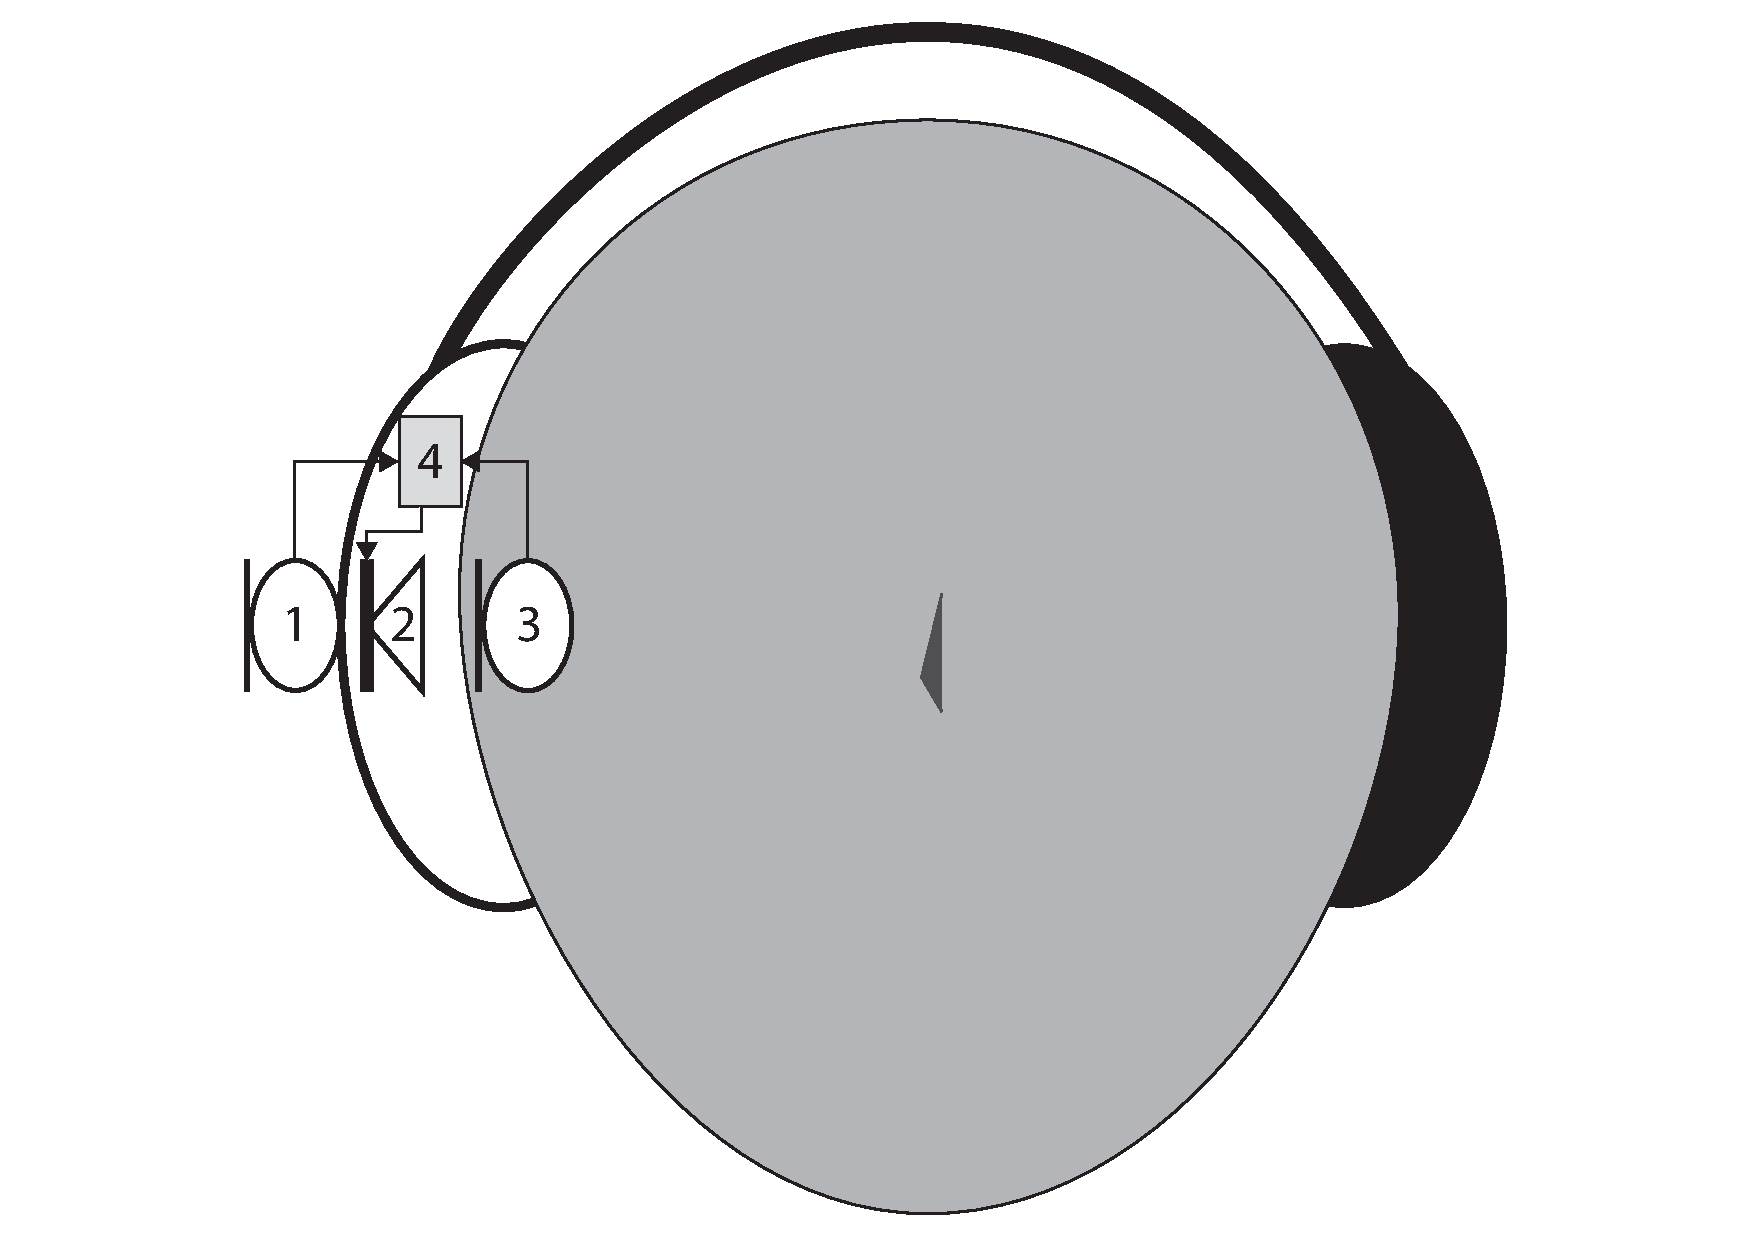
\includegraphics[width=1\columnwidth]{figures/ArticleIllustrations/SystemOverview}
%	\caption{System Overview}
%	\label{fig:SystemOverview}
%\end{figure}



\subsection{Feedforward ANC using FXLMS}
%The adaptive feedforward ANC system is shown on \autoref{fig:ANCFeedforward}


The system in \autoref{fig:ANCFeedforward} outputs a control signal $y[n]$, which ideally is a counter-phase signal of the noise. The signal is generated by inputting the reference signal $x[n]$ into a control filter consisting of adaptive coefficients $b[z]$ representing the transfer function from the reference microphone to the headphone loudspeaker. The coefficients are adapted using the FXLMS algorithm. The FXLMS algorithm inputs the filtered reference $f[n]$ signal along with the error signal $e[n]$. The filtered reference signal is used combined with the error signal to determine new optimal coefficients for the control filter, this is shown in equation \ref{eq:FXLMS}. The signals from (1)(3) are converted to the digital domain using an ADC and anti aliasing filters (AA) before processing. When processed, the output $y[n]$ is reconstructed and converted using a DAC.

 \vspace{-4mm}
{
	%\centering
	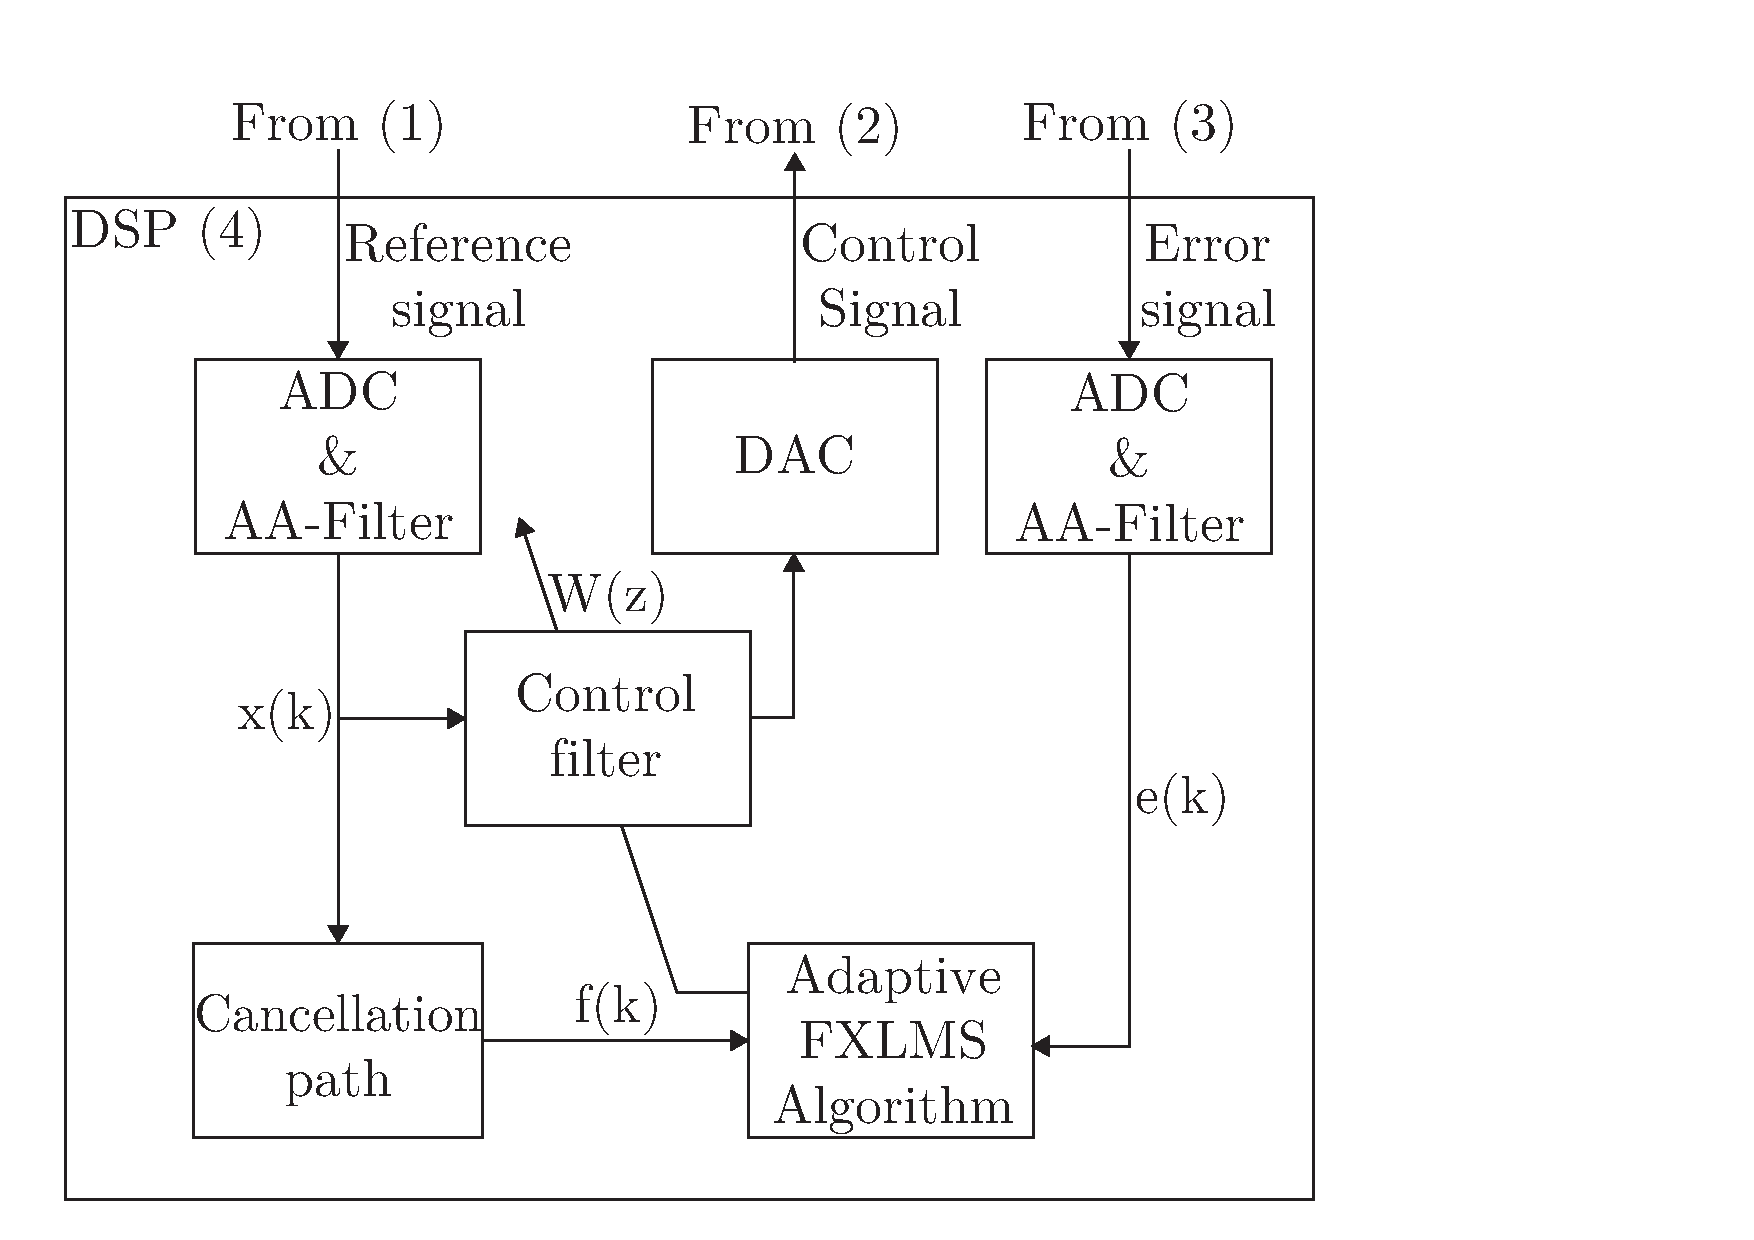
\includegraphics[width=1\columnwidth]{figures/ArticleIllustrations/ANCFeedForward}
	\captionof{figure}{Adaptive feedforward ANC system.}
	\label{fig:ANCFeedforward}
}

%\begin{figure}[H]
%	\centering
%	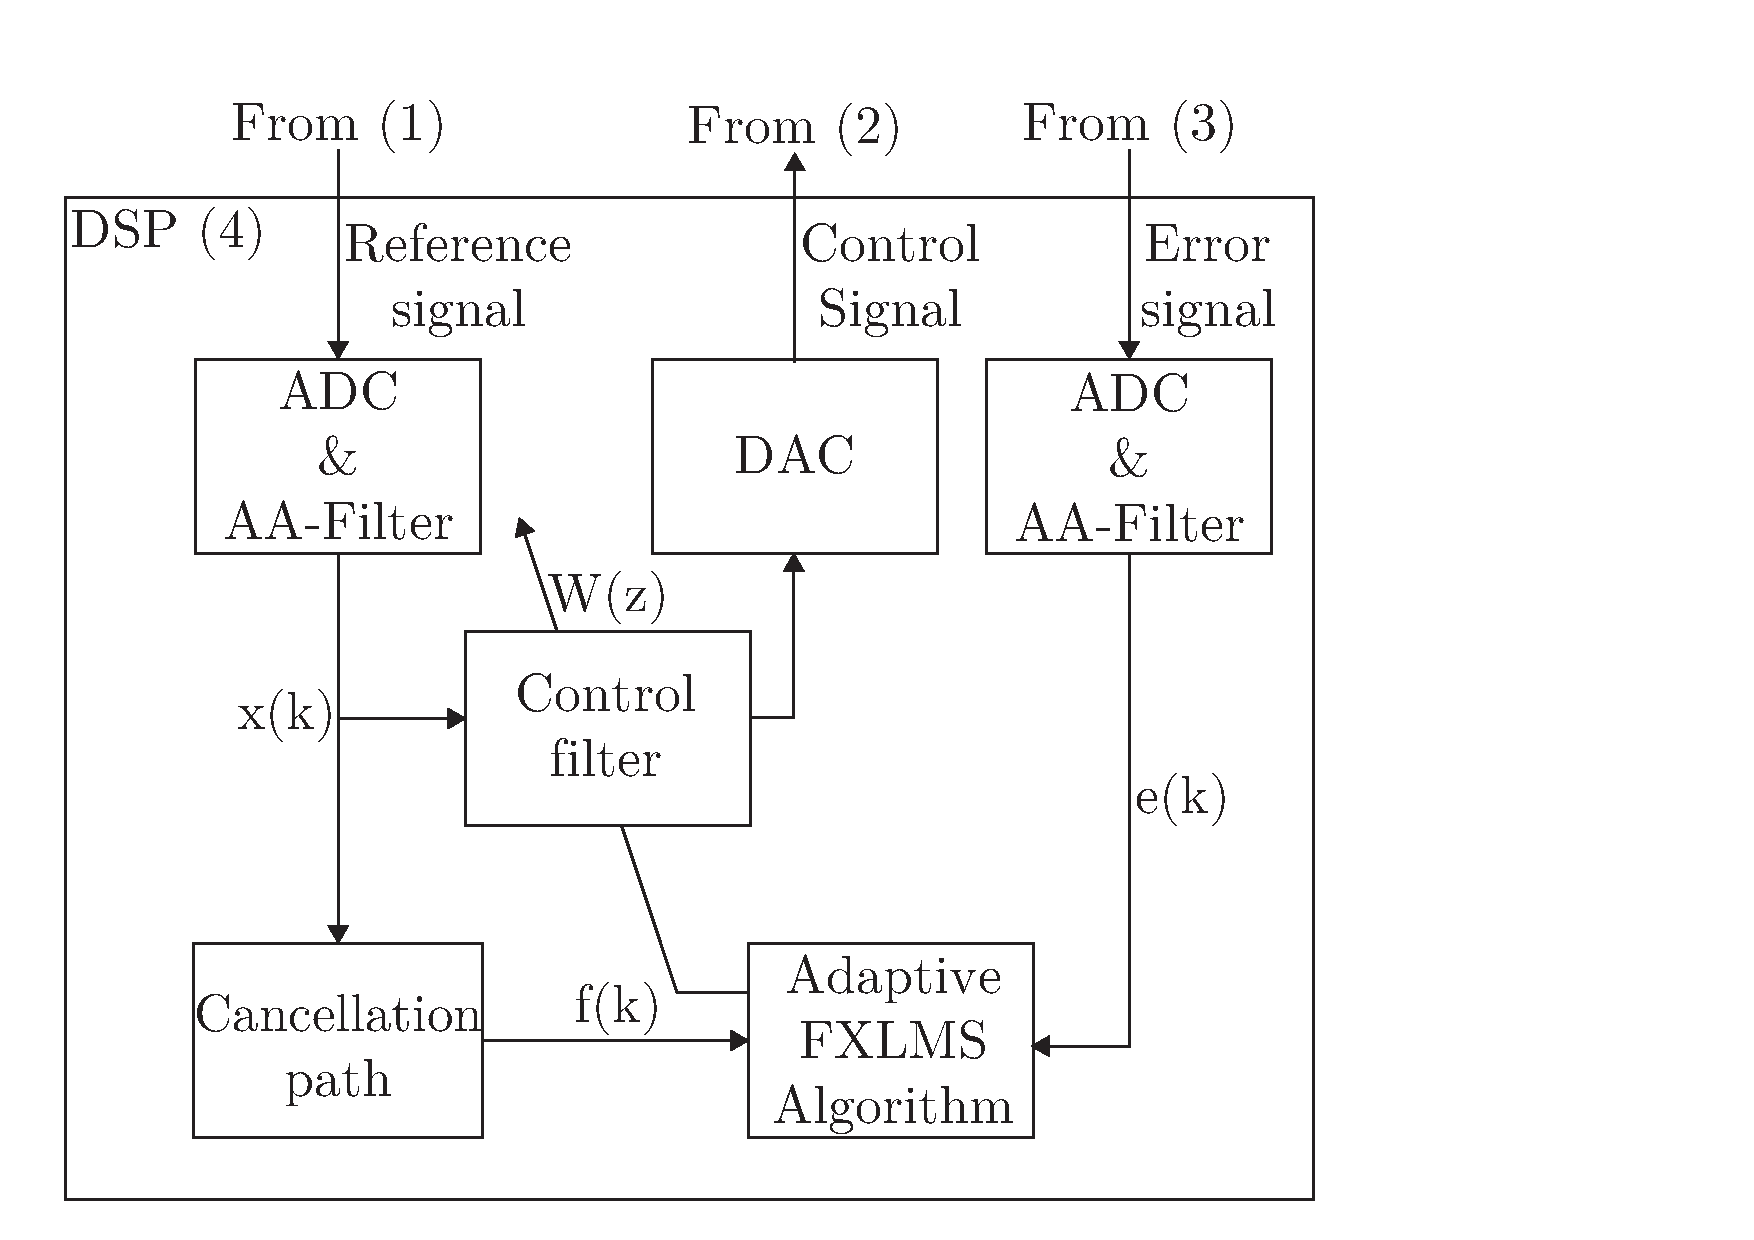
\includegraphics[width=1\columnwidth]{figures/ArticleIllustrations/ANCFeedForward}
%	\caption{Adaptive feedforward ANC system}
%	\label{fig:ANCFeedforward}
%\end{figure}


\textbf{Control Filter} The filter, shown in equation \ref{eq:Output}, is initialized with the inverse of the measured impulse response of the represented transfer function. An order of 256 taps is chosen based on subjective testing in simulation.
\vspace{-3mm} % yeah I know - Sorry Mikkel!
\begin{equation}\label{eq:Output}
y[n]=\sum_{j=0}^{L-1}b_j[n]x[n-j]
\end{equation}
where $b_j[n]$ is the weight coefficients written as  $b[n]=[b_0[n],b_1[n], \cdots, b_{L-1}[n]]^T$.

\textbf{FXLMS} is the optimization algorithm which updates the control filter coefficients using the FXLMS method shown in \autoref{eq:FXLMS}.
\begin{equation}\label{eq:FXLMS}
b_j[n+1] = b_j[n] - 2\mu e[n]f[n-j]
\end{equation}
where $\mu$ is the convergence factor, $e[n]$ is the error and $f[n]$ is the reference convolved with the Cancellation Path.

\textbf{Cancellation Path} (CP) is the transfer-function from the headphone loudspeaker to the error microphone. In the literature \cite{Hansen} the CP is adaptively adjusted, but it is assumed constant because the position of the headphone does not change while measured on a Head and Torso Simulator (HATS). This assumption is made because it is irrelevant for verifying if LP is a plausible solution. 


%When implementing the system, delays exist due to the anti-aliasing and reconstruction filters. The delays of the system exceeds the propagation time of sound from the reference microphone to the headphone loudspeaker resulting in poor performance. Therefore an LP-algorithm is proposed to predict future samples in order to decrease the effect of the time delays.

\subsection{Characteristics of Speech}
Speech can be split into two main classes, voiced and unvoiced. Voiced sounds are characterized by a strong periodicity, with the fundamental frequency referred to as the pitch frequency (50 - 500 Hz). Unvoiced sounds are characterized as random. Speech is a non stationary signal and can only be assumed Wide Sense Stationary (WSS) for periods of 20 - 30 ms \cite{Speech}. 

\subsection{Linear Prediction of Speech}
In order to predict future samples the Auto Correlation Function (ACF), used in LP, of speech must be estimated in frames. The outlines of the prediction system is shown in figure \ref{fig:LinearPredictionOverview}.

\begin{figure}[H]
	\centering
	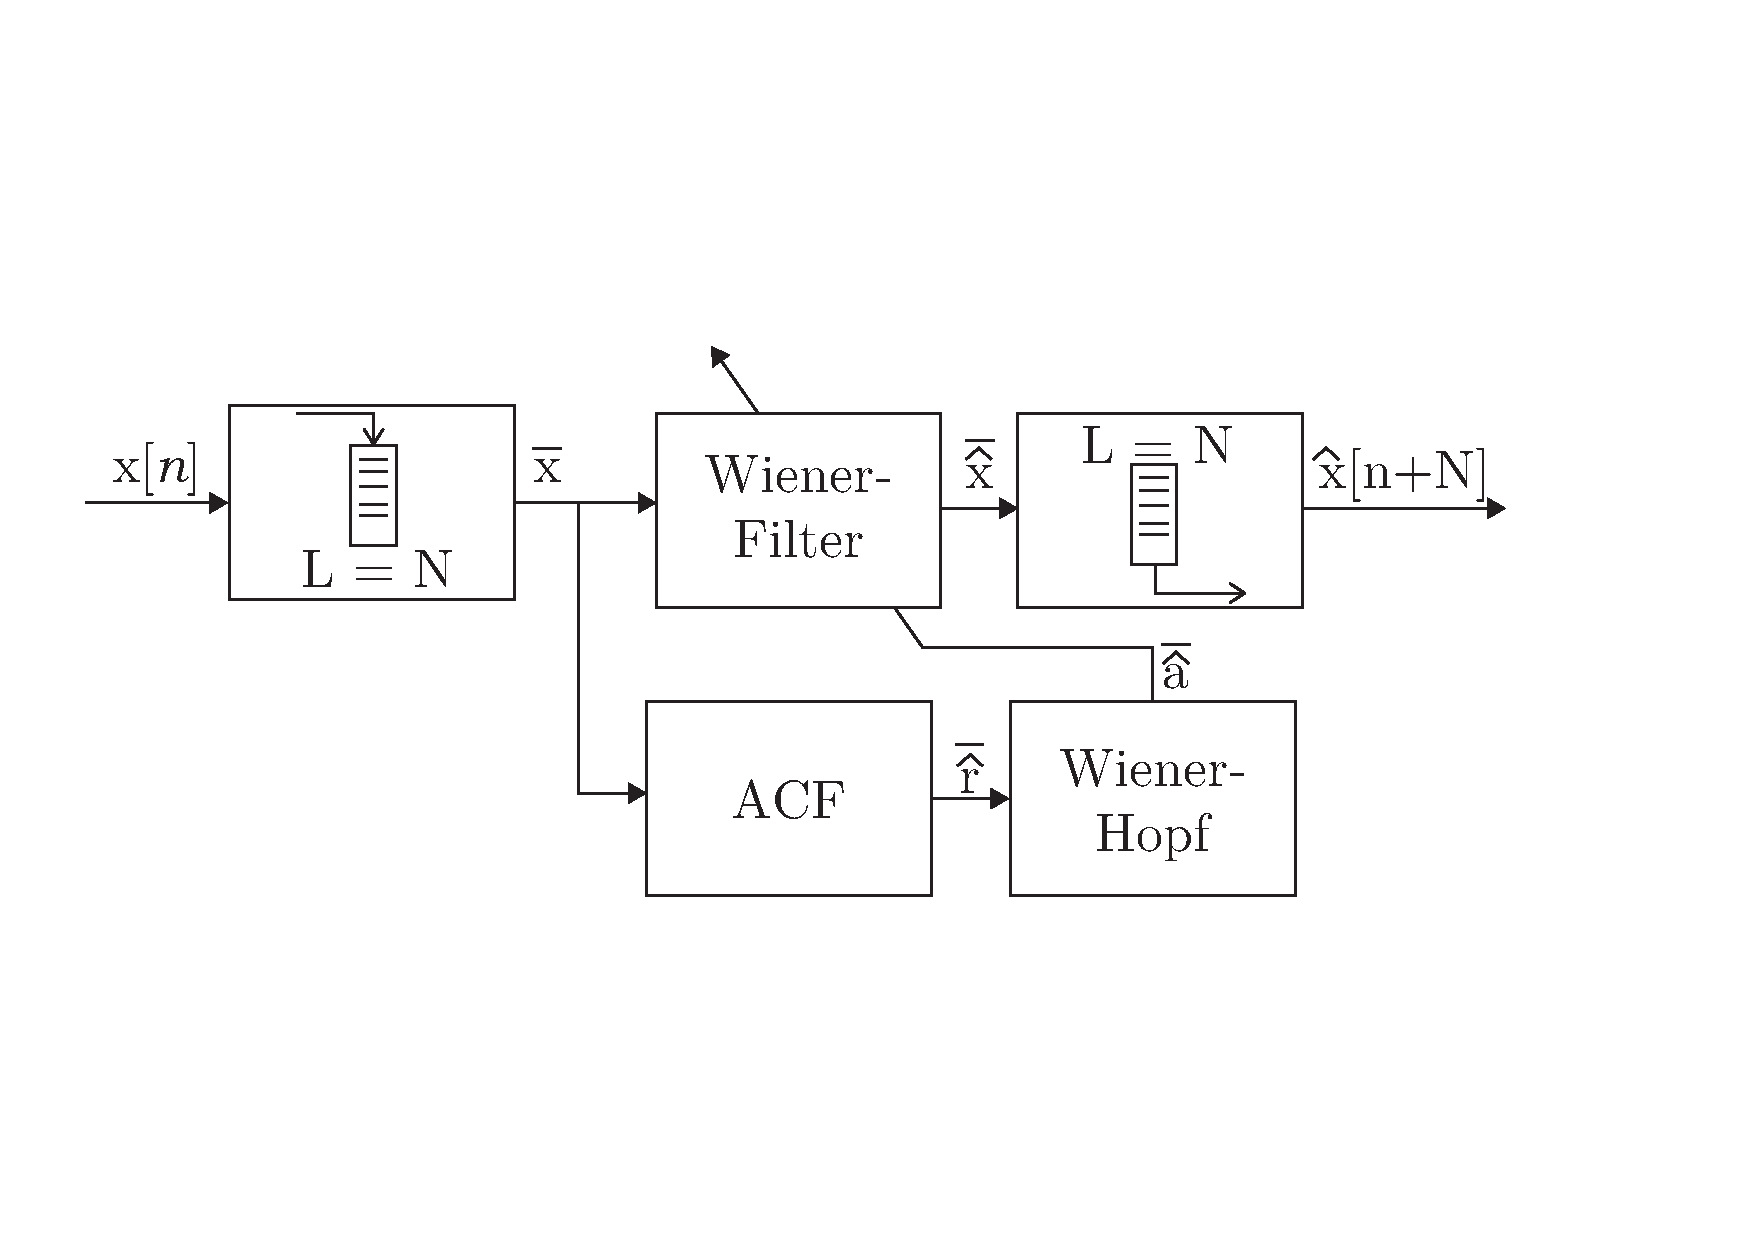
\includegraphics[width=\columnwidth]{ArticleIllustrations/WienerHopf}
	\caption{Linear prediction system.}
	\label{fig:LinearPredictionOverview}
\end{figure}


Utilizing a nonrecursive estimation of the ACF, shown in \autoref{eq:nonrecursive}, it is possible to determine the linear prediction coefficients $\hat{\bar{a}}$ (LPCs) used for predicting future samples \cite{LinearPrediction}. When estimating the ACF of the input ($x$) a Hamming window ($w$) is applied.
\begin{equation}\label{eq:nonrecursive}
%%r_x[l,m] = \sum^{m}_{n=m-N+1+\left| l\right|} x_l[n]w_l[m-n]
\hat{r}_x[l] = \sum^{N}_{n=\left| l\right|} x_l[n]w_l[N-n]
\end{equation}
%\begin{multline}\label{eq:nonrecursive}
%R[l,m] = \sum^{m}_{n=m-N+1+\left| l\right|} \\ x[n]w[m-n] x[n-\left| l\right|]w[m-n+\left| l\right|]
%\end{multline}
%\begin{equation}
%R[l,m]=\sum^{m}_{n=m-N+1+\left| l\right|}x[n]w[m-n] x[n-\left| l\right|]w[m-n+\left| l\right|]
%\end{equation}
where $x_l[n]=x[n]x[n-l]$, $w_l[n]=w[n]w[n+l]$, $l$ is the lag and $N$ is the frame size.

The LPCs are determined using \autoref{eq:normal}, known as the Wiener-Hopf equation.
\begin{equation}\label{eq:normal}
\hat{R}  \bar{a} = -\bar{\hat{r}}_x
\end{equation}
where $\hat{R}$ is the covariance matrix $\hat{C}_{xx}$, $\bar{\hat{a}}$ is the LPCs $\bar{\hat{a}} = [\hat{a}_1 , \hat{a}_2, \cdots, \hat{a}_N]^T$ and $\bar{\hat{r}}_x$ is the ACF, $\bar{\hat{r}}_x = [\hat{r}_x[1] , \hat{r}_x[2], \cdots, \hat{r}_x[N]]^T$.

\autoref{eq:normal} can be rewritten as shown in \autoref{eq:normal2} yielding the LPCs directly.  
 \begin{equation}\label{eq:normal2}
\bar{\hat{a}} = \hat{-R^{-1}} \bar{\hat{r}}_x
\end{equation}
Calculating $\hat{R^{-1}}$ is computationally heavy on a DSP. To estimate the LPCs the Levinson-Durbin method is used \cite{LinearPrediction}. Prediction using Wiener filtering, shown in equation \ref{eq:Predictor}, can then be applied to the current frame for prediction of the next frame. 

\begin{equation}\label{eq:Predictor}
\hat{x}[n+1] =- \sum^{N}_{i=1}\hat{a}_ix[n-i]
\end{equation}

Using equation \ref{eq:Predictor} in cascade where $\hat{x}[n+2]$ is estimated using $\hat{x}[n+1]$ and $x[n]$. The predicted frame is then used as input for the ANC system.

\subsection*{Feedforward LP FXLMS}


\section*{Results}
\subsection{Prediction Gain}
For the purpose of testing LP prediction gain (PG) shown in \autoref{eq:PG} will be used. 
\begin{equation}\label{eq:PG}
PG = 10 log_{10}\bigg(\frac{\sigma^2_x}{\sigma^2_\varepsilon}\bigg) = 10 log_{10}\bigg(\frac{E\{x^2[n]\}}{E\{\varepsilon^2[n]\}}\bigg)
\end{equation}
where PG is the ratio between the variance of the input signal $x[n]$ and the variance of the prediction error $\varepsilon$ in (dB). The higher the PG the better the prediction is.



\subsection{Determining System Parameters}
The parameters which should be detemined are $fs$, $P$, $N$, $O$, and $M$ using \autoref{eq:PG}.         
The PG of variable $fs$ is shown on \autoref{fig:fsPredict}.

\begin{figure}[H]
	\centering
	\textbf{\textit{Here is going to be a graph of PG determined by fs}}
	\caption{PG }
	\label{fig:fsPredict}
\end{figure}


%These are detemined respectively using a Prediction Gain ($PG$) to find the optimum value. 
The PG of variable $N$, $O$ and $M$ is seen on \autoref{fig:PredictParameters}. 
\begin{figure}[H]
	\centering
	\textbf{\textit{Here is going to be a graph of PG determined by N}}
	\textbf{\textit{Here is going to be a graph of PG determined by O}}
	\textbf{\textit{Here is going to be a graph of PG determined by M}}
	\caption{PG }
	\label{fig:PredictParameters}
\end{figure}

\subsection{Simulation of Feedforward LP FXLMS}

\begin{figure}[H]
	\centering
	\tikzsetnextfilename{DelayRatio}
	% This file was created by matlab2tikz.
%
%The latest updates can be retrieved from
%  http://www.mathworks.com/matlabcentral/fileexchange/22022-matlab2tikz-matlab2tikz
%where you can also make suggestions and rate matlab2tikz.
%
\definecolor{mycolor1}{rgb}{0.00000,0.44700,0.74100}%
\definecolor{mycolor2}{rgb}{0.85000,0.32500,0.09800}%
%
\begin{tikzpicture}

\begin{axis}[%
width=3in,
height=1.75in,
scale only axis,
xmin=0,
xmax=50,
xmajorgrids,
xlabel={Delay [100 $\times$ samples]},
ymin=0,
ymax=70,
ylabel style={yshift=0.3em},
xlabel style={yshift=-0.2em},
ytick={0,10,...,70},
ymajorgrids,
ylabel={Attenuation [dB]},
xticklabel shift={.1cm},
yticklabel shift={.1cm},
axis background/.style={fill=white}
]
\addplot [color=mycolor2,solid,line width=1.5pt,forget plot]
  table[row sep=crcr]{%
2	66.5420250310586\\
4	52.9717264302022\\
6	49.4175149424998\\
8	46.8717703569681\\
10	47.5886347675082\\
12	48.5221420089092\\
14	36.1913078215459\\
16	24.6480360536532\\
18	18.5625963047043\\
20	15.9345988709594\\
22	15.2225924490026\\
24	14.4941735350858\\
26	13.5145912190769\\
28	12.5242379572864\\
30	11.8400523957144\\
32	11.4203165228037\\
34	11.2428861871564\\
36	11.1050592495872\\
38	10.862823901561\\
40	10.6158645117455\\
42	10.3154480278615\\
44	9.97867799972119\\
46	9.61958031033587\\
48	9.31052791122033\\
50	9.08997582022533\\
};
\addplot [color=mycolor1,line width=1.5pt,solid,forget plot]
table[row sep=crcr]{%
	2	25.5751628128288\\
	4	20.0199680852144\\
	6	17.0442763613153\\
	8	15.1060127156582\\
	10	13.7310612019933\\
	12	12.6685774343164\\
	14	11.7903474171974\\
	16	11.0441690144364\\
	18	10.3883064900616\\
	20	9.78797702825996\\
	22	9.23075404560805\\
	24	8.7110676592604\\
	26	8.22176906503967\\
	28	7.77006791263877\\
	30	7.35426684398216\\
	32	6.94907270624338\\
	34	6.5323972441528\\
	36	6.08060777493347\\
	38	5.57101511941803\\
	40	4.99733350616245\\
	42	4.35167702165293\\
	44	3.61433096515684\\
	46	2.757705271237\\
	48	1.74470077738877\\
	50	0.5254168140125\\
};
\end{axis}
\end{tikzpicture}%
	\caption{Attenuation achieved by the system for different system delays.}
	\label{Fig:Reference to noise ratio}
\end{figure}








% At this point in time all results are not yet certain, however we will give an idea of how they are going to turn out.
% As presented in the paper thus far, we know what kind of noise we would like to cancel out and how we want to do it. The following list tells which graph will be used to show the results of the acceptance tests.

% \begin{itemize}
% \item Prediction gain - The difference between the input signal and the estimated signal, measured in dB. Used in the LP part.
% \item A plot comparison of frequency response between: A pure signal, a signal with FXLMS noise attenuation and a signal with LP combined with FXLMS attenuation
% \item An expansion of \autoref{Fig:Reference to noise ratio}: As of now only attenuation is showed, but in the future another graph in the figure will show the attenuation of the FXLMS combined with LP - which should yield better attenuation at larger delays.

% \end{itemize}




%\vspace{5in}
  \begin{itemize}
  	\item The AAU poster theme v. 1.1.0 has been tested with baposter v. 2.0, and it can be downloaded from my AAU website \cite{jknaau} or my personal website \cite{jknsqrt-1}.
  	\item If you find a bug in the AAU theme (and not in the baposter template), please do not hesitate to contact me. There is a FAQ at the baposter website \cite{baposter}, if you should have any problems with it.
<<<<<<< HEAD
  \end{itemize}
  
  
%\begin{figure}
%  	\floatbox[{\capbeside\thisfloatsetup{capbesideposition={left,top},capbesidewidth=4cm}}]{HammingNOP10}[\FBwidth]
%  	{\caption{A test figure with its caption side by side}\label{fig:test}}
%  	{\includegraphics[width=5cm]{name}}
%\end{figure}
=======
  \end{itemize}
>>>>>>> 386cdecef39d26e2fa621022e6bf7b02f6531c34


\bibliography{00setup/mybib}
% that's all folks
\end{document}


